\section{深度优先遍历}
\label{sec:graph-dfs}

广度优先遍历同时推进许多条路线，每条只走一步。另一种访问方式是只盯住一条路线：从当前顶点走向一个尚未见过的邻居，再从那里继续往前，直到无路可走才退回上一个顶点，改走它的下一个邻居。走迷宫时用左手扶墙一路前进、碰到死路再折回，就是这种方式。它天然地维持着“当前正在走的这条分支”，因而能判断沿当前分支是否绕回了自己，也能记录每个顶点何时把所有出路都探完。本节建立这一过程，并说明这两条信息分别有什么用。

\subsection{栈与递归访问}
\label{sec:graph-trav-dfs-stack}

\paragraph{三种状态与栈帧}
沿分支前进时，一个顶点经历三个阶段：尚未被走到，称为未发现；已经走到、但它的邻居还没有检查完，称为处理中；邻居全部检查完毕、不会再从它出发，称为已完成。区分后两种状态是必要的，因为“已经见过”并不等于“已经处理完”。处于处理中的顶点恰好构成从本次起点到当前位置的一条分支，用一个后进先出的栈保存：栈底是起点，栈顶是当前顶点。

只记住栈中的顶点还不够。退回到某个顶点时，需要接着检查它的下一个邻居，而不是从头再来。因此栈中的每一帧保存一个顶点$u$，以及$u$的邻接表中下一条待检查记录的位置。另外用父指针$p(v)$记录$v$是从哪个顶点走过来的。这种访问方式称为深度优先遍历，也常称\term{深度优先搜索}（depth-first search，DFS）。

\begin{algorithm}[深度优先遍历（显式栈）]
\label{alg:graph-trav-dfs}
输入：图$\mathcal G=(V,E)$的邻接表。输出：父指针、每个顶点的发现时刻$d(v)$与完成时刻$f(v)$。
\begin{enumerate}
  \item 所有顶点置为未发现，时钟$t=0$。按某个固定次序扫描顶点；每遇到一个未发现的顶点$r$，令$p(r)$为空，执行下面两步。
  \item 发现$r$：$t\gets t+1$，$d(r)=t$，$r$改为处理中，把帧$(r,\text{邻接表起点})$压入栈。
  \item 当栈非空时，看栈顶帧$(u,\text{位置})$。若$u$还有未检查的邻居，读取下一个邻居$v$（有向图只读出邻居），并把位置后移一格：$v$未发现时，置$p(v)=u$，$t\gets t+1$，$d(v)=t$，$v$改为处理中并压入新帧；$v$处于处理中或已完成时，不压栈，继续下一轮。若$u$的邻居已全部检查，则$t\gets t+1$，$f(u)=t$，$u$改为已完成并弹出栈顶帧。
\end{enumerate}
\end{algorithm}

用递归写，同样的过程更短：访问$u$时先记发现时刻，然后对每个未发现的邻居$v$置$p(v)=u$并递归访问$v$，所有邻居处理完后记完成时刻。递归调用时，程序运行时会自动保存“$u$检查到了第几个邻居”，这正是显式栈中每一帧记录的位置。两种写法的访问次序完全一样。

\paragraph{完整执行过程}
图~\ref{fig:graph-trav-dfs-stack}(a)是一个有分支的有向图，弧为$1\to2$、$1\to5$、$2\to3$、$2\to4$、$5\to4$。从$1$出发并按编号读取出邻居：发现$1$，再发现$2$，再发现$3$；$3$没有出邻居，于是完成$3$并弹栈，回到$2$。$2$的下一个出邻居$4$未发现，压栈；$4$也没有出邻居，完成后回到$2$，此时$2$的邻居已检查完，完成$2$。回到$1$，它的下一个出邻居$5$未发现，压栈；$5$唯一的出邻居$4$已经完成，不再压栈，$5$随即完成；最后完成$1$，栈变空。图~\ref{fig:graph-trav-dfs-stack}(b)画出了每个事件之后的栈，黄色格子是栈顶。

\begin{figure}[!htb]
  \centering
  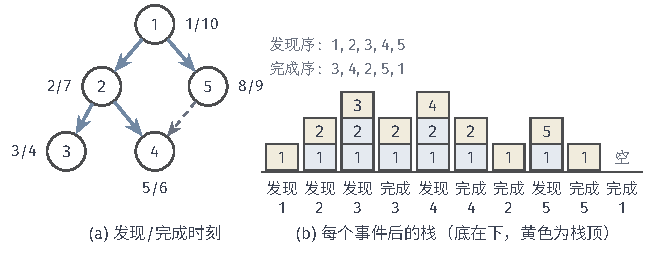
\includegraphics[width=109.8mm]{figures/01-basic-mathematics/04-graphs/tikz/c2-dfs-stack-trace/figure.pdf}
  \caption{有向图$1\to2$、$1\to5$、$2\to3$、$2\to4$、$5\to4$上从$1$出发的深度优先遍历，出邻居按编号读取。(a)顶点旁的“$d/f$”是发现时刻与完成时刻，蓝色箭头是父指针对应的弧，虚线弧$5\to4$检查时$4$已完成。(b)十个事件后的栈，底在下、栈顶为黄色；栈高上升对应发现，下降对应完成。}
  \label{fig:graph-trav-dfs-stack}
\end{figure}

若栈空时仍有未发现的顶点，算法回到第一步，从下一个未发现顶点重新开始。已经完成的顶点保持原状态，不会被重新访问。这样，整次执行把每个顶点恰好发现一次、完成一次；父指针把顶点组织成若干棵有根树，称为深度优先森林。只在发现时处理顶点，得不到“何时探完”的信息，因此完成事件要单独记录，下一小节会看到它的用处。

\paragraph{计算开销}
每个顶点恰好压栈一次、弹栈一次；每一帧的位置只向后移动，所以每条邻接记录恰好被读取一次。邻接表下总时间为$O(n+m)$，状态、时刻、父指针和栈占$O(n)$额外空间。栈的深度等于当前分支上的顶点数，最坏可达$n$：在一条长链$1\to2\to\cdots\to n$上，栈会一直增长到装下全部顶点。递归实现时，这意味着递归深度也是$n$，可能超出程序运行环境允许的调用深度；显式栈把这部分存储放在普通数组中，避免这一问题。

\subsection{发现次序与完成次序}
\label{sec:graph-trav-dfs-orders}

\paragraph{两种次序}
按发现时刻从小到大排列顶点，得到\term{发现次序}（discovery order）；按完成时刻排列，得到\term{完成次序}（finishing order）。在图~\ref{fig:graph-trav-dfs-stack}中，发现次序是$1,2,3,4,5$，完成次序是$3,4,2,5,1$。两种次序的差别来自栈的结构：一个顶点被发现之后，在它弹栈之前压入的所有顶点都位于它上方，必须先弹出。所以一个顶点的后代全部先于它完成，而它自己最后完成；$2$的后代$3,4$先完成，然后才轮到$2$。

下面两个引理把这一观察写准确。第一个说明时刻区间怎样嵌套，第二个说明哪些顶点一定会成为后代；第~\ref{sec:graph-connectivity-computation}节计算强连通分量、第~\ref{sec:graph-topological-order}节构造拓扑次序时都要用到它们。

\begin{lemma}[时刻区间的嵌套]
\label{lem:graph-trav-dfs-nesting}
在一次完整的深度优先遍历中，若顶点$v$在$u$处于处理中时被发现，即$d(u)<d(v)<f(u)$，则$v$是$u$在深度优先森林中的后代，且$f(v)<f(u)$。
\end{lemma}

\begin{proof}
$v$被发现时压入栈，位于$u$的上方，因为此时$u$仍在栈中。栈后进先出，$v$必须在$u$之前弹出，所以$f(v)<f(u)$。另外，$v$的父指针指向发现它时的栈顶，这个栈顶要么是$u$，要么是在$u$之后压入的顶点；对后者重复同样的推理，父指针链只会经过$u$上方的顶点，最终到达$u$。因此$v$是$u$的后代。
\end{proof}

\begin{lemma}[未发现路径]
\label{lem:graph-trav-white-path}
若在时刻$d(u)$存在一条从$u$到$v$的路径（有向图中沿弧方向），路径上除$u$以外的顶点此时都未发现，则$v$最终成为$u$的后代，从而$f(v)<f(u)$。
\end{lemma}

\begin{proof}
假设结论不成立，在路径上取第一个不成为$u$后代的顶点$w$，记它在路径上的前一个顶点为$x$。$x$是$u$本身或$u$的后代，所以$f(x)\leq f(u)$。$x$在完成之前要检查弧$x\to w$，因此$w$在$f(x)$之前已被发现；而按假设$w$在$d(u)$时尚未发现，所以$d(u)<d(w)<f(x)\leq f(u)$。由引理~\ref{lem:graph-trav-dfs-nesting}，$w$是$u$的后代，矛盾。
\end{proof}

\paragraph{共享后继：发现次序不能代替完成次序}
设图~\ref{fig:graph-trav-dfs-stack}中的弧表示依赖，$i\to j$意味着$i$要排在$j$之前。顶点$4$同时是$2$和$5$的后继。若按发现次序$1,2,3,4,5$安排，$5$排在$4$之后，违反了弧$5\to4$：发现$4$时走的是经过$2$的分支，发现次序完全没有反映$5$也指向它。完成次序则不同。$4$在$5$之前就已完成，反转完成次序得到$1,5,2,4,3$，逐条检查五条弧都是起点在前。第~\ref{sec:graph-trav-dfs-toposort}节会证明，在无环图中这一做法总是成立。

\paragraph{父路径一般不是最短路线}
深度优先遍历的父指针同样给出从根到每个顶点的路线，但它反映的是“沿哪条分支先走到”，与距离无关。在贯穿四点图上从$1$出发、按编号读取邻居：$1$走到$2$，$2$的第一个未发现邻居是$3$，$3$的未发现邻居是$4$，于是父路径为$1\to2\to3\to4$，有三条边；而$1\to2\to4$只需两条边，$1$与$3$甚至直接相邻。需要最少边数时，应使用广度优先遍历。

\subsection{环的检测与恢复}
\label{sec:graph-trav-cycle-detection}

\paragraph{有向图：指向栈内顶点的弧}
处理中的顶点构成当前分支，并且父指针已经把它们按先后串成一条有向路径。若在检查栈顶$u$的出邻居时遇到弧$u\to v$，而$v$也处于处理中，那么沿父指针从$u$往回走一定会到达$v$，这段路径与弧$u\to v$合起来就是一个有向环。这样的弧称为\term{回边}（back edge）。图~\ref{fig:graph-trav-cycle-detection}(a)中，栈内依次是$1,2,3$，检查$3\to1$时$1$仍在栈中，沿父指针$3\to2\to1$回溯，再补上$3\to1$，得到有向环$1\to2\to3\to1$。

指向已完成顶点的弧不能这样处理。图~\ref{fig:graph-trav-cycle-detection}(b)中先走$1\to2$，$2$没有出邻居而完成；回到$1$后走到$3$，检查$3\to2$时$2$已完成。$2$已经不在当前分支上，弧$3\to2$无法与当前分支拼成环。本例中从$2$出发也回不到$3$（否则由引理~\ref{lem:graph-trav-white-path}，$3$会在$2$完成之前就被发现），图中确实没有环。一般地，指向已完成顶点的弧本身不提供成环的证据；图中若另有环，下面的定理保证遍历会在别处遇到回边。只看“是否已经访问过”会把这种情形误判为环，这正是要区分处理中与已完成的原因。

\begin{figure}[!htb]
  \centering
  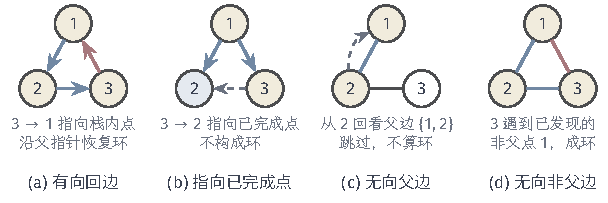
\includegraphics[width=102.9mm]{figures/01-basic-mathematics/04-graphs/tikz/c2-dfs-cycle-detection/figure.pdf}
  \caption{深度优先遍历中环的判断。黄色为处理中（在栈内）的顶点，蓝色填充为已完成顶点，蓝色粗线为父指针对应的边。(a)有向图中$3\to1$指向栈内顶点，构成回边，沿父指针恢复出环；(b)$3\to2$指向已完成顶点，不构成环；(c)无向图中从$2$回看父边$\{1,2\}$，这是同一条边的反向查看，应当跳过；(d)无向三角形中$3$遇到已发现、但不经父边相连的顶点$1$，构成环（红色）。}
  \label{fig:graph-trav-cycle-detection}
\end{figure}

\begin{theorem}[有向环的判定]
\label{thm:graph-trav-directed-cycle}
有限有向图含有向环，当且仅当对它的一次完整深度优先遍历中出现回边。出现回边$u\to v$时，父指针链$v\to\cdots\to u$加上弧$u\to v$就是一个有向环。
\end{theorem}

\begin{proof}
充分性已在上面说明：$v$处于处理中且$u$是当前栈顶，$u$在$v$上方，由引理~\ref{lem:graph-trav-dfs-nesting}$u$是$v$的后代，父指针链给出从$v$到$u$的有向路径。

必要性。设图含有向环，在环上取最先被发现的顶点$v$，记环上指向$v$的弧为$u\to v$。在时刻$d(v)$，环上其余顶点都未发现，沿环从$v$走到$u$的路径满足引理~\ref{lem:graph-trav-white-path}的条件，所以$u$成为$v$的后代，$d(v)<d(u)<f(u)<f(v)$。$u$在完成之前要检查弧$u\to v$，那时$v$尚未完成，仍处于处理中，因此$u\to v$是一条回边。
\end{proof}

\paragraph{无向图：跳过实际的父边}
无向图中每条边在两端的邻接表里各出现一次。从$u$走到$v$之后，$v$检查邻居时会再次看到$u$，这只是同一条边的反向记录，不是新的路线。若把它当作“遇到已发现顶点”，任何一条边都会被误判为环，如图~\ref{fig:graph-trav-cycle-detection}(c)。因此规则是：检查$u$的一条邻接记录$e=\{u,w\}$时，若$e$就是使$u$被发现的父边，跳过；否则只要$w$已经被发现，就报告存在环。图~\ref{fig:graph-trav-cycle-detection}(d)中，$3$经父边与$2$相连，它看到的$1$已被发现、且不经父边相连，于是$1\text{--}2\text{--}3\text{--}1$是一个环。允许平行边时，要按边的身份跳过，只跳过实际作为父边的那一条；两点之间的另一条平行边会与父边构成长度为$2$的环。

这一规则在两个方向上都可靠。若整次遍历从未报告，每条边在两端被检查时，要么发现了新顶点而成为父边，要么正是父边的反向记录，所以所有边都是父边，图就是深度优先森林本身，没有环。反过来，考察第一次报告时的边$e=\{u,w\}$，可以说明$w$此时一定在栈中。假设$w$已完成。$w$完成之前检查过$e$：若那时$u$未发现，$u$会成为$w$的后代并先于$w$完成，与$u$此刻仍在处理相矛盾；若那时$u$已发现，那次检查本身就该报告，除非$e$是$w$的父边，而这意味着$u$当初已经通过$e$发现了$w$，不会现在才第一次读到$e$。于是$w$是栈中位于$u$下方的祖先，父指针链从$w$到$u$再加上$e$构成一个环；由于$e$不是$u$的父边，在简单图中这个环至少有三个顶点。算法既给出了“有环”的结论，也给出了这个环本身，可以直接核对。
